\chapter{段路由航点生成算法实验验证}

\section{引言}

本章将通过基于 \gls*{P4} 的 \gls*{BMv2} 实现特定报文转发流程,使用 \gls*{SRv6} 作为验证的 \gls*{SR} 标准协议,验证前两章提出的段路由航点生成算法。 \gls*{P4} 是一种协议无关的数据包处理流程编程语言,研究人员可以用编程的方式定义报文转发流程。首先,需要编写可以转发 \gls*{SRv6} 的数据面处理逻辑,包括 \gls*{SRv6} 的封装,解封装和移动段指针;其次,编写两种算法下的控制面;再者,构造数据中心拓扑和运营商拓扑;最后,进行打流实验并最终得出实验结论。

\section{实验环境}

1. 实验拓扑环境

本实验使用 \gls*{BMv2} 作为软件交换机。使用基于IPv6的段路由作为段路由标准而不是基于标签预留协议的段路由,因为IPv6是未来IP网络的趋势。而且基于IPv6的段路由使用128位的SID,更具有可编程性和可扩展性。本实验使用Linux命名空间(namespace)来隔离网络堆栈,使用 \gls*{veth} 来模拟交换机之间的接口。基于IPv6的段路由程序用 \gls*{P4} 语言开发,在 \gls*{BMv2} 上加载实现,控制器的功能则由一个python进程来实现,整体实验架构如图5-1所示。

\begin{figure}[htbp]
\setlength{\abovecaptionskip}{15pt plus 3pt minus 2pt}
\centerline{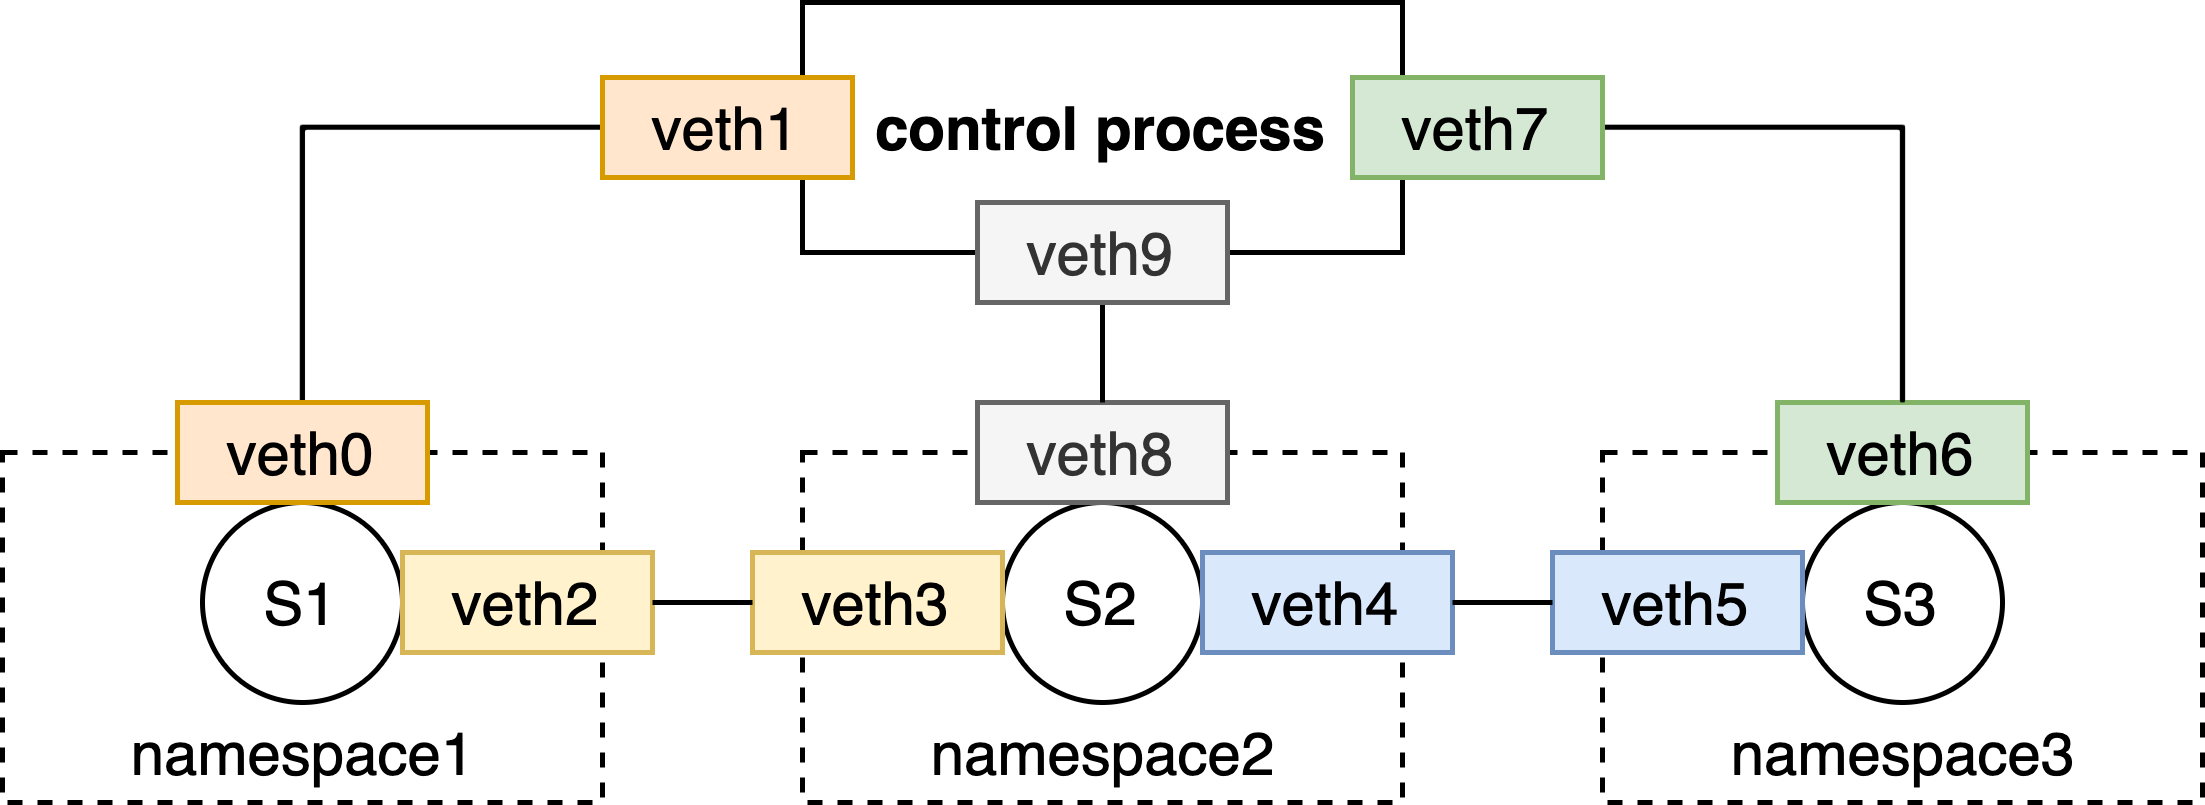
\includegraphics[width=0.8\textwidth]{./figures/ch3-test-env.png}}
\caption{实验环境示意图}
\label{fig-ch3-test-env}
\end{figure}

2. 集中式算法仿真实现

第三章提出的集中式段路由航点选择算法在实验验证中由python实现。控制器主进程内运行有三个主要线程,第一个是用于检测网络拓扑变化的网络事件监听线程,第二个是给段路由节点下发段路由表项、给非段路由节点下发普通转发表项、计算链路权重和辅助图等拓扑事件驱动信息的标签分发、链路权重及辅助图计算线程,第三个是接收流量时延请求,运行航点列表生成算法并将计算结果下发给首节点的段路由航点列表计算线程。

\begin{figure}[htbp]
\setlength{\abovecaptionskip}{15pt plus 3pt minus 2pt}
\centerline{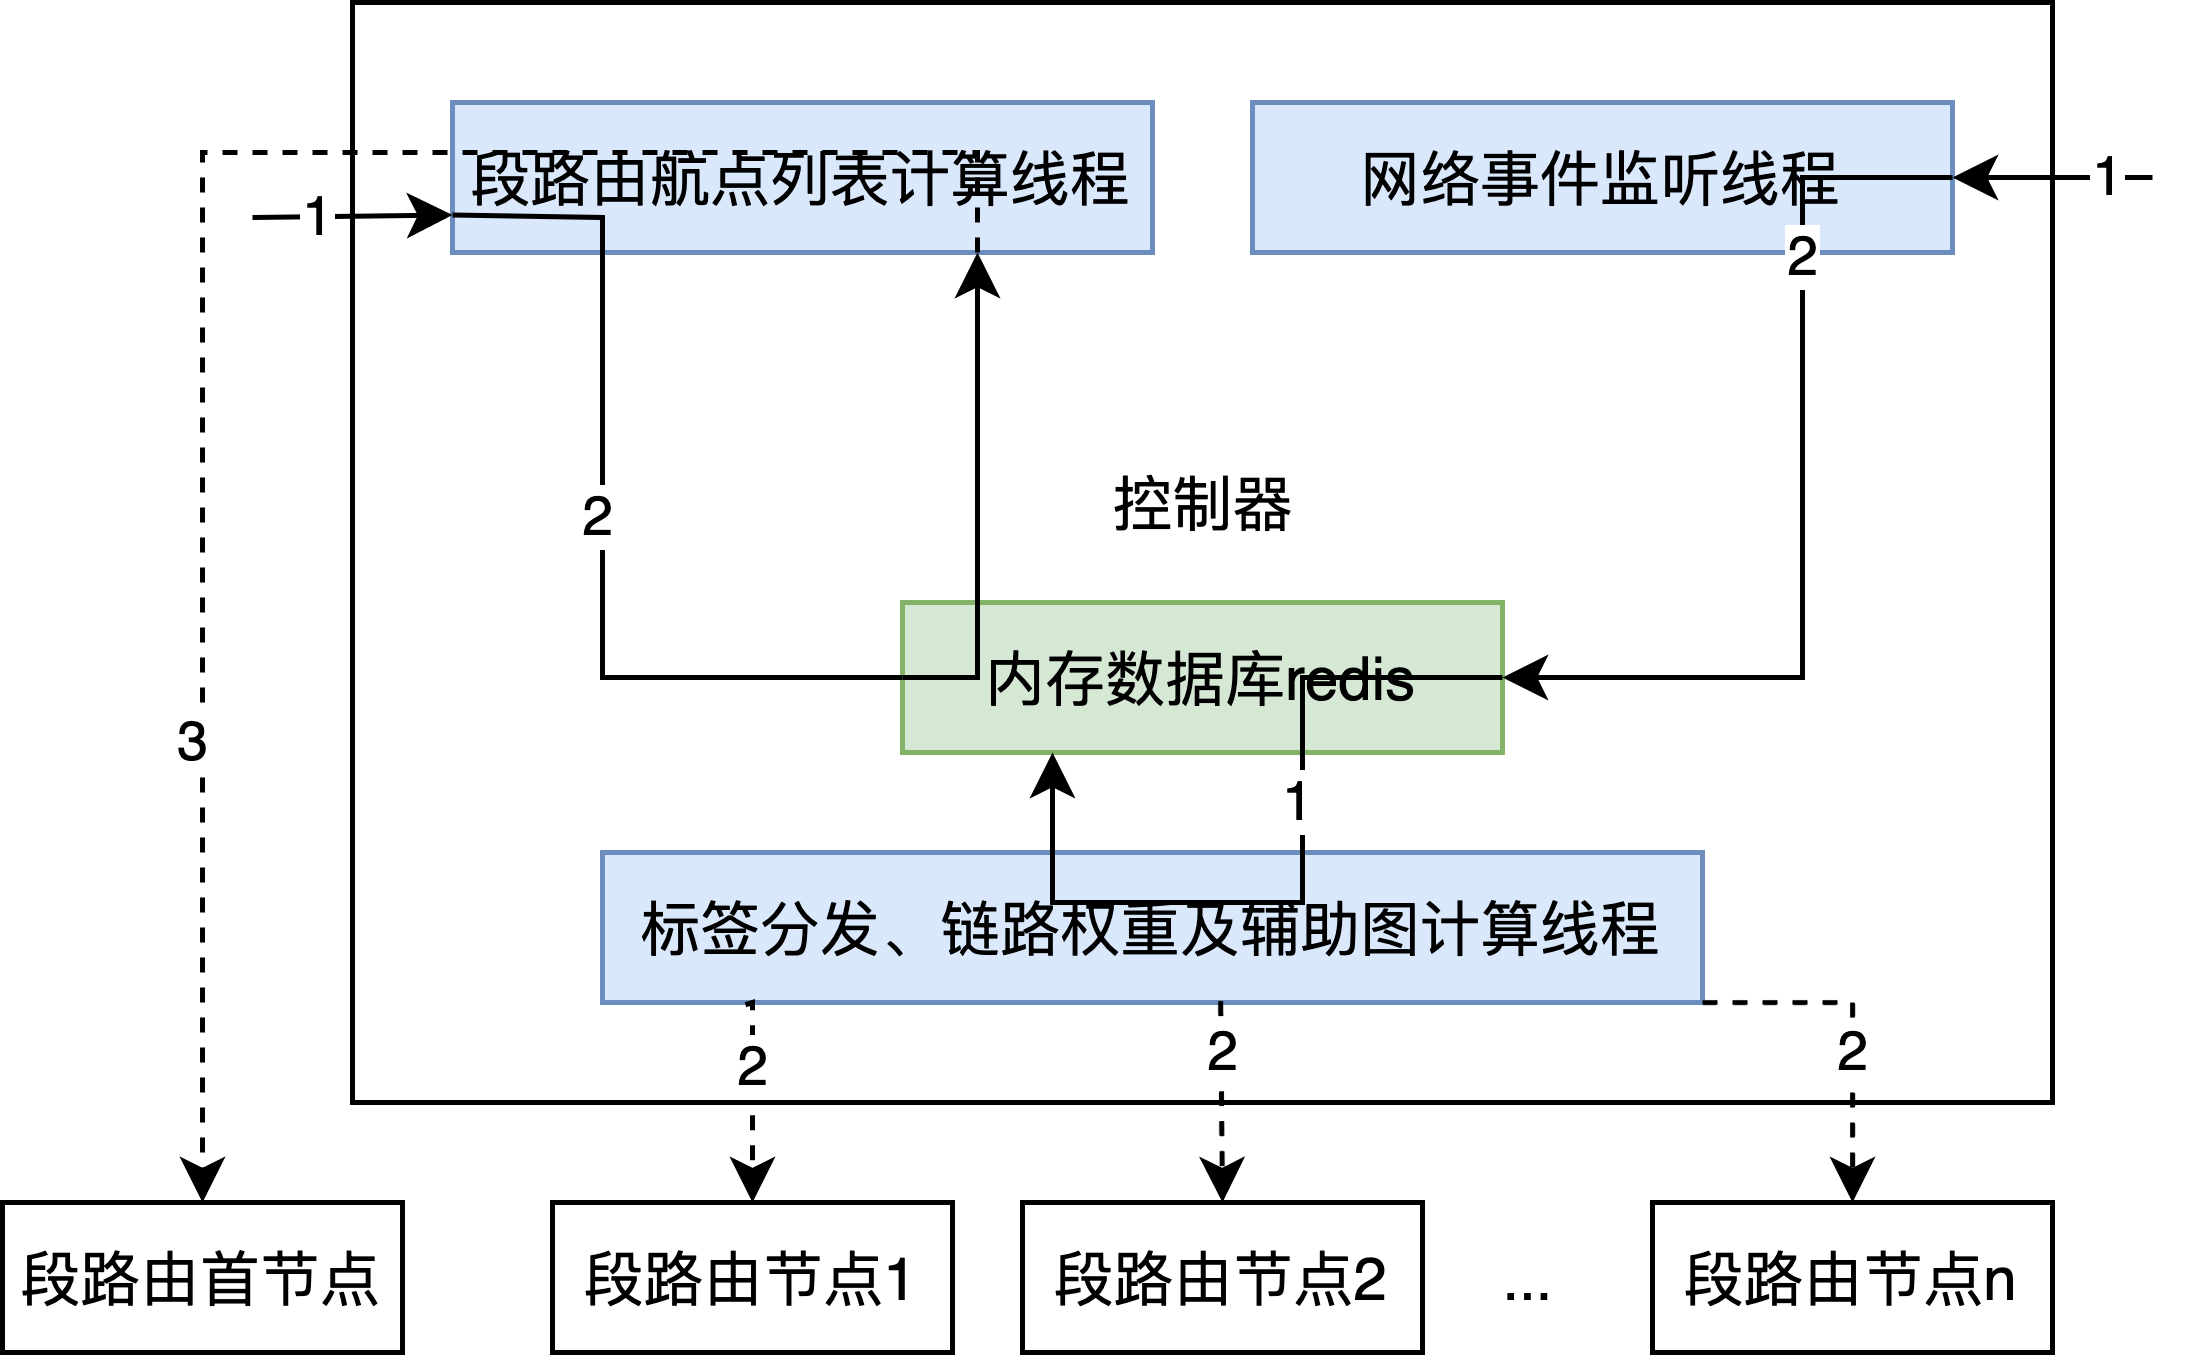
\includegraphics[width=0.8\textwidth]{./figures/ch3-test-code.png}}
\caption{集中式算法代码结构示意图}
\label{fig-ch3-test-code}
\end{figure}

整个实验实现架构如图5-2所示:网络事件监听进程由网络事件触发,第一步接收到网络变更的信号,第二步将变化后的网络信息填在内存数据库中。标签分发、链路权重及辅助图计算线程由检测数据库的管道触发,第一步查看拓扑更新的信息,第二步判断是否需要更新段路由标签,如果需要变化段路由标签则下发新的标签到段路由设备上,计算变化后拓扑的链路权重并重新生成辅助图。段路由航点列表计算线程由从段路由首节点发来的业务请求报文嗅探接口触发,第一步接受业务报目标地址和目标时延的需求,第二步通过段路由航点列表生成算法生成段路由航点列表,第三步将生成的段路由航点标签列表作为流表下发给段路由首节点。

3. 分布式算法仿真实现

第四章提出的分布式段路由航点选择算法在实验验证中由python实现。段路由节点主进程内运行有三个主要线程,第一个是用于对探测列表内段路由节点进行时延探测并更新时延矩阵的线程,第二个是接收其他段路由节点通告时延矩阵结论并更新时延矩阵的线程,第三个是对服务流量进行航点列表生成算法的线程。段路由节点的探测目标节点列表由控制器生成,通过管理配置的方式下发给段路由节点。

\begin{figure}[htbp]
\setlength{\abovecaptionskip}{15pt plus 3pt minus 2pt}
\centerline{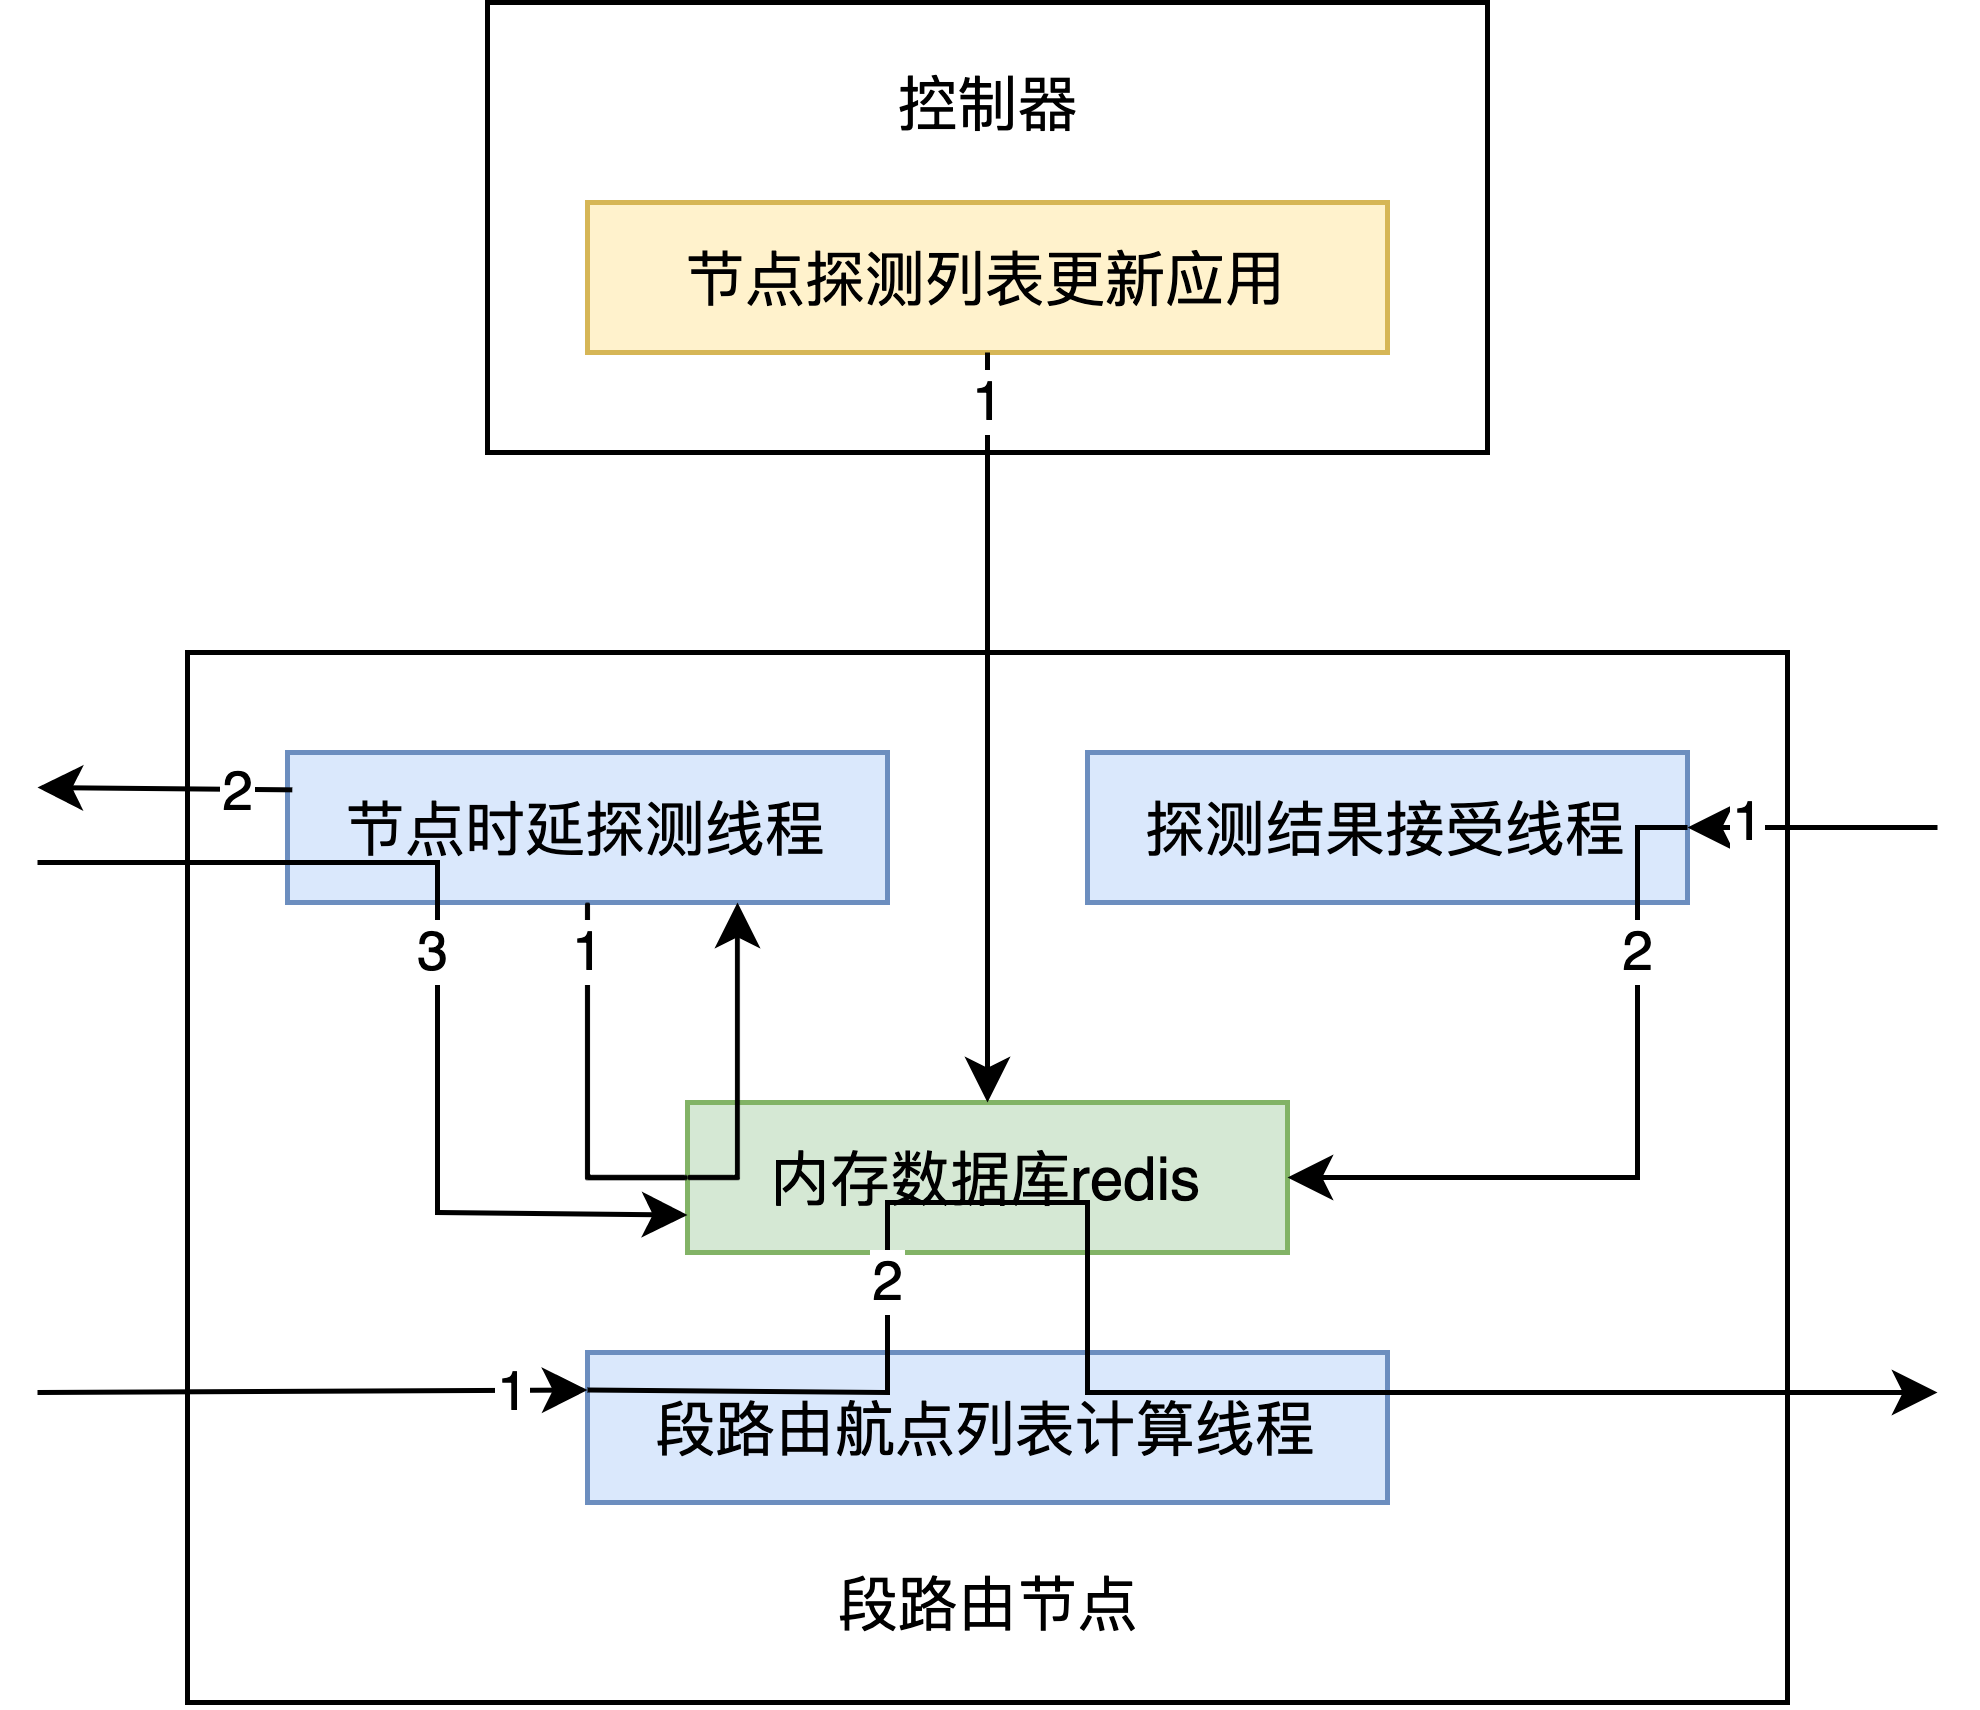
\includegraphics[width=0.8\textwidth]{./figures/ch4-test-code.png}}
\caption{分布式算法代码结构示意图}
\label{fig-ch4-test-code}
\end{figure}

整个实验实现架构如图5-3所示:节点时延探测线程由计时器触发,第一步从内存数据库中获取需要进行时延探测的节点列表,第二步对外进行时延探测并记录结果,第三步将采集的结果与内存数据库中的差分时延矩阵数据进行比较并按照更新算法进行更新。探测结果接收线程由本节点的公告报文嗅探机制接收到其他段路由节点发送来的报文这一事件触发,第一步接收公告报文并处理报文内容,第二步将发布节点公告的时延的信息按照实验矩阵更新算法在内存数据库中进行更新。段路由航点列表计算线程由本节点的业务报文嗅探机制接收到带有目标时延请求的报文这一事件触发,第一步接受业务报文并提取目标地址和目标时延,第二步通过段路由航点列表生成算法生成段路由航点列表。

\section{段路由基础功能实验}

本节实验用于测试段路由的基本功能,包括段路由包头和段列表封装、段路由包头弹出、段路由转发功能。

\subsection{实验步骤}

启动如图5-4的三节点线性网络拓扑,$h1$发包,$h3$收包,其中$h1$节点需要封装段路由航点列$<S2, S3>$,$S2$将段指针加1,$S3$弹出段路由报文头和段列表,进而转发给$h3$。

\begin{figure}[htbp]
\setlength{\abovecaptionskip}{15pt plus 3pt minus 2pt}
\centerline{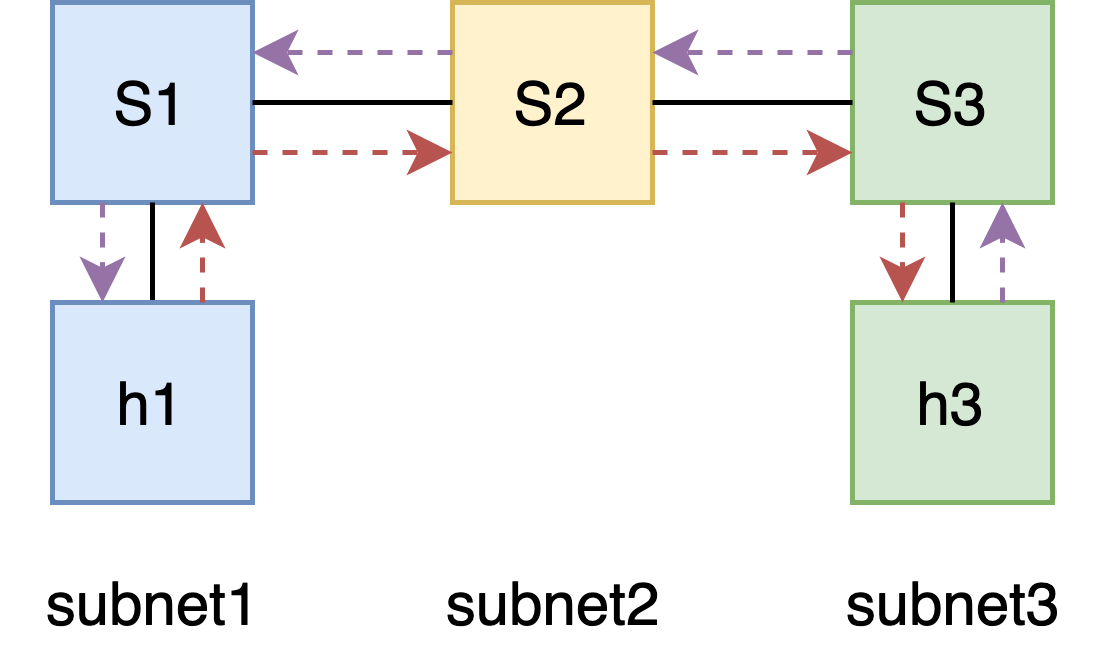
\includegraphics[width=0.6\textwidth]{./figures/ch5-three-line-topo.png}}
\caption{三节点线性网络拓扑图}
\label{fig-ch5-three-line-topo}
\end{figure}

1. 启动网络拓扑,新建3个网络命名空间,每一个网络命名空间相当于一个子网。将每对 \gls*{veth} 绑定到对应的网络命名空间上并分配IPv6地址。将设计好的拓扑中的每个 \gls*{BMv2} 启动,加载编译的 \gls*{P4} 二进制文件,并的各个端口绑定到 \gls*{veth} 上,这样在每对 \gls*{veth} 间就形成连接两个 \gls*{BMv2} 的链路。

2. 启动控制器,控制器将通过thrift接口和 \gls*{BMv2} 建立带外通路进行控制流量传输。控制器将给所有虚拟交换机下发基础转发表项,包括二层广播表,等价多路径路由哈希组表,三层IPv6的路由器广告、邻居通告等代答表和三层IPv6路由表,使得全网拓扑中的节点可以用IPv6地址互通。集中式算法下控制器需要继续和虚拟交换机保持连接,分布式算法下控制器则可以断开连接,控制器在分布式场景下仅起到配置初始化表项的作用。

3. 检查$S1$的表项,确定其包含以下表项$srv6\_transit$表:目标地址为$fdbd:0:33::/48$的报文会被封装为$<fdbd:0:22:22::,\ fdbd:0:33:33::>$;检查$S3$的表项,确定其包含目标地址为$fdbd:0:11::/48$的报文会被封装为$<fdbd:0:22:22::,\ fdbd:0:11:11::>$的 $srv6\_transit$表;检查$S2$和$S3$的表项,确定其包含$srv6\_my\_sid$表:目标地址为自己段标签的报文会进行$srv6\_end$操作,即:

\lstset{
    numbers=left, 
    numberstyle= \tiny, 
    keywordstyle= \color{ blue!70},
    commentstyle= \color{red!50!green!50!blue!50}, 
    frame=shadowbox, % 阴影效果
    rulesepcolor= \color{ red!20!green!20!blue!20} ,
    escapeinside=``, % 英文分号中可写入中文
    xleftmargin=2em,xrightmargin=2em, aboveskip=1em,
    framexleftmargin=2em
}
\begin{lstlisting}
hdr.srv6h.segment_left = hdr.srv6h.segment_left - 1;
hdr.ipv6.dst_addr = local_metadata.next_srv6_sid;
\end{lstlisting}


最终弹出整个段路由报文头的动作直接由 \gls*{P4} 流水线完成,不用放置到$table$里。各个节点表项如表5-1所示.

\begin{table}[]
\begin{tabular}{|l|l|l|l|l|}
\hline
段路由节点 & 表项名称 & 匹配字段 & 动作 & 动作参数 \\ \hline
\multirow{2}{*}{\textbf{S1}} & \textbf{srv6\_transit} & \textbf{fdbd:0:33::/48} & \textbf{srv6\_t\_insert\_2} & \textbf{\textless{}fdbd:0:22:22::, fdbd:0:33:33::\textgreater{}} \\ \cline{2-5} 
    & \textbf{srv6\_my\_sid} & \textbf{fdbd:0:11:11::} & \textbf{srv6\_end} &  \\ \hline
\textbf{S2} & \textbf{srv6\_my\_sid} & \textbf{fdbd:0:22:22::} & \textbf{srv6\_end} &  \\ \hline
\multirow{2}{*}{\textbf{S3}} & \textbf{srv6\_transit} & \textbf{fdbd:0:11::/48} & \textbf{srv6\_t\_insert\_2} & \textbf{\textless{}fdbd:0:22:22::, dbd:0:11:11::\textgreater{}} \\ \cline{2-5} 
    & \textbf{srv6\_my\_sid} & \textbf{fdbd:0:33:33::} & \textbf{srv6\_end} &  \\ \hline
\end{tabular}
\caption{段路由基础功能测试节点表项表}
\label{table-sr-entries}
\end{table}

4. 从$h1$的发送 \gls*{Ping} 报文到$h3$,报文正常转发,且每一步转发都符合 \gls*{SRv6} \cite{SRARK} 标准的要求。

\subsection{实验结论}

实验证明,用本节提出的仿真模型可以进行段路由报文的处理,可以进一步下发特定段路由航点列表进行算法性能验证。

\section{组网流量调度实验}

本小节将对第三章、第四章提出的两种时延保障段路由航点生成算法进行实验验证,实验将分别构建基于树形拓扑的数据中心网络拓扑和基于随机生成的运营商网络拓扑,并在这些拓扑中验证两个算法和各自对照组的时延保障效果。其中第三章集中式段路由航点生成算法的对照组是基于带宽信息生成段路由航点列表的算法;第四章分布式段路由航点生成算法的对照组是基于最短路径的传统分布式网络选路算法。

\subsection{算法实验步骤}

第一步启动网络拓扑,新建若干个网络命名空间,每一个网络命名空间相当于一个子网。在网络命名空间间绑定 \gls*{veth} 形成连接两个虚拟交换机的链路。并将虚拟交换机启动加载 \gls*{P4} 二进制文件使得每个节点具有段路由的基础功能。

第二步启动控制器,控制器将给所有虚拟交换机 \gls*{BMv2} 通过带外通路下发基础表项,包括二层广播表,等价多路径路由哈希组表,三层IPv6的路由器广告、邻居通告等代答表和三层IPv6路由表,使得全网拓扑中的节点可以用IPv6地址互通。

第三步在网络中选择两组相隔较远的节点,开始用流量生成软件Iperf持续性打流,保证在实验阶段网络处于有流量的动态状态。Iperf是一个用于网络性能测量和调优的工具。它是一种跨平台工具,可以为任何网络生成标准化的性能测量。Iperf具有客户端和服务器功能,并且可以创建数据流来测量两端之间的一个或两个方向的吞吐量。典型的 Iperf 输出包含传输的数据量和测量的吞吐量的时间戳报告,本研究对时延结果数据的采集就是通过时间戳来获取。

第四步区分集中式控制和分布式控制:

\begin{itemize}
\item 集中式控制下调整段路由航点选择算法参数,并启动段路由航点选择算法应用,为针对时延敏感流量进行段路由航点选择做好准备。
\item 分布式控制下启动每台虚拟交换机的分布式控制应用。控制应用将初始化内存数据库中每个节点的时延探测列表,段路由节点中的探测结果接收线程和段路由航点列表计算线程将开始监听各个绑定 \gls*{veth} 的端口嗅探公告时延数据包和服务请求数据包。准备好为流量进行段路由航点选择。
\end{itemize}

第五步选择一组源节点和目的节点开始从小流量开始打流,直到开始发生大规模的丢包,记录每次增加流量后控制器算法应用计算分配出的航点和端到端的时延情况。

第六步分析整理数据,得出结论。

\subsection{实验结果分析}

1. 集中式段路由航点生成算法实验结果分析

\begin{figure*}[t] %, height=3.2cm
\centering
\hspace{0.00\linewidth}
\subfloat[$\alpha$取值测试结果图]{
    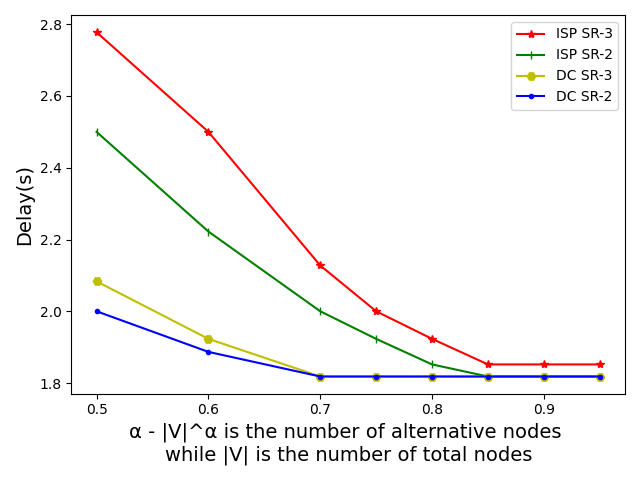
\includegraphics[width=0.46\linewidth]{./figures/ch3-test-1.png}
    \label{fig-ch3-test-1}
}
\hspace{0.00\linewidth}
\subfloat[平均延迟实验结果图]{
    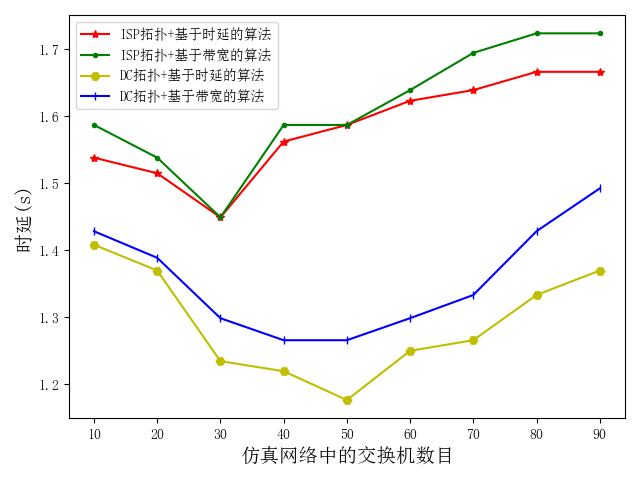
\includegraphics[width=0.46\linewidth]{./figures/ch3-test-2.png}
    \label{fig-ch3-test-2}
}
\\
\hspace{0.00\linewidth}
\subfloat[标签列表长度实验结果图]{
    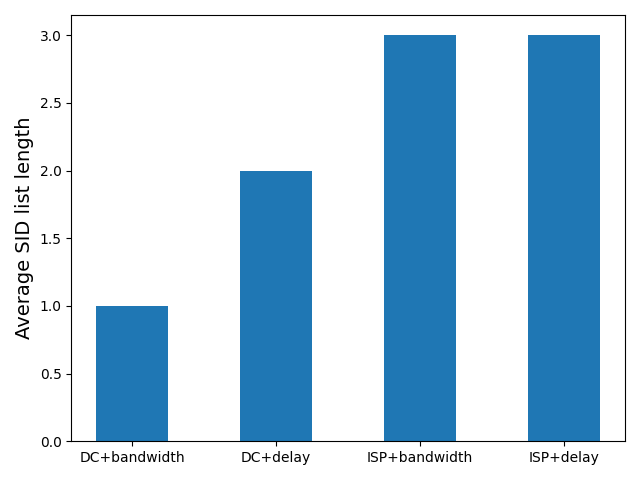
\includegraphics[width=0.46\linewidth]{./figures/ch3-test-3.png}
    \label{fig-ch3-test-3}
}
\hspace{0.00\linewidth}
\subfloat[保证请求延迟要求比例测试结果图]{
    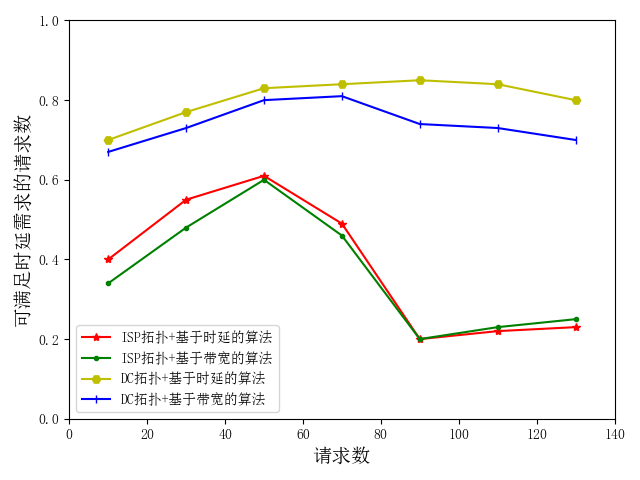
\includegraphics[width=0.46\linewidth]{./figures/ch3-test-4.png}
    \label{fig-ch3-test-4}
}
\caption{集中式段路由航点列表生成算法实验结果图} 
\label{fig:test:centralised}
\end{figure*}

图5-5是集中式段路由航点生成算法针对参数取值、时延保障效果、段路由列表长度的实验结果。

\begin{itemize}
\item (a)是$\alpha$取值测试结果。为了验证候选节点占原拓扑全部节点的比率$\alpha$的取值。该试验将选择两个拓扑,一个是数据中心的树状拓扑结构,一个是随机生成的互联网服务提供商(ISP)拓扑。两个拓扑都具有40个节点;另外分别将段路由标签列表限制为2跳或3跳,即$SR-2$和$SR-3$。每一次确定参数$\alpha$的取值后后按照实验步骤3开始打流,记录iperf打流的时延结果。图中横轴是$\alpha$的大小,纵轴是延迟。

在数据中心的树状拓扑结构中,根据$SR-2$、$SR-3$进行比较,同时调整$\alpha$的值。可以看出,当选择$\alpha=0.7$时,在数据中心场景中SR-2和SR-3的情况下可以达到最佳值。其含义是:当节点集中有节点中心度在前${|V|}^{0.7}$的节点时。需要在计算中考虑时,已经可以得到效果最优的段路由路径。而在互联网服务提供商拓扑中,使用随机拓扑进行模拟,在$SR-2$和$SR-3$的情况下,$\alpha=0.85$可以达到最优值。

\item (b)是平均延迟实验结果图,该实验是为了验证在同样使用贝尔曼-福特算法作为标签列表选择核心算法的前提下,采用本文提出的链路权重以及生成辅助图的方案和直接用链路带宽作为权重的方案进行比较。实验的对照组同样是数据中心的树状拓扑结构和随机生成的互联网服务提供商拓扑。本实验的自变量是网络的大小,用网络拓扑中的交换机数目,即节点数目做为横坐标,因变量是打流的时延结果,并将其在纵坐标上描点,进而分析得出结论。图(b)表明,当使用考虑时延的链路权重进行段路由标签列表计算时,无论使用树状拓扑结构还是随机拓扑结构,相对于直接使用带宽信息来计算来段列表,都能获得更低的平均延迟。
\item (c)是段路由航点生成算法下对所生成标签列表的长度进行记录的实验。这是为了验证3.3.1中提到的用段路由标签列表的长度被用来限制段列表生成算法,在数据中心的树状拓扑结构和互联网服务提供商随机拓扑结构中,分别使用了本文提出的基于带宽的贝尔曼-福特算法,以及本文提出的参考延迟的贝尔曼-福特算法。对四种场景下生成的段路由标签列表的平均列表长度进行比较。横坐标是四种测试场景,纵坐标是段标签列表的长度。本文提出的算法倾向于使用稍大的段列表长度,但考虑到贝尔曼-福特算法在生成段列表长度的时候会对长度进行限制,所以可以通过约束条件来保障段标签列表长度不会太长。本文使用的段标签列表都是2个或3个,因此可以认为没有产生额外的段列表标签开销。
\item (d)是保证请求延迟要求比例测试。该实验室为了验证使用本文提出的参考时延属性的段路由标签列表生成算法是否可以对时延需求进行保障。本实验的对比拓扑还是树状拓扑和互联网服务提供商拓扑,分别使用本文提出的参考延迟的贝尔曼-福特算法和基于带宽的贝尔曼-福特算法来计算给定服务请求数在10、50、90、130的情况下,可以分别保证请求延迟要求的比例。横坐标自变量是发起请求的数目,在实验中是从不同的源地址到目的地址进行打流,查看该流量被调度后的时延是否符合目标时延的需求,即实际时延小与目标时延,对满足时延需求的请求进行计数,与总请求数的比例就是纵坐标的数据。到可以看出,无论在树状拓扑结构还是互联网服务提供商拓扑中,本研究提出的算法都具有更好的延迟保证效果。
\end{itemize}

2. 分布式段路由航点生成算法实验结果分析

\begin{figure*}[t] %, height=3.2cm
\centering
\hspace{0.00\linewidth}
\subfloat[树状拓扑下与边界网关协议对时延需求保障的比较结果图]{
    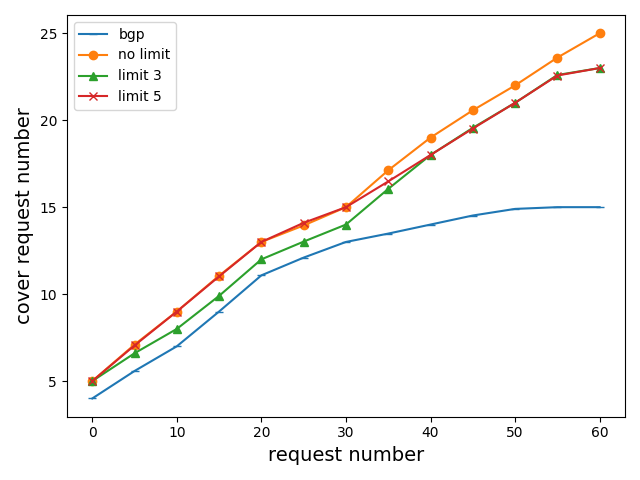
\includegraphics[width=0.46\linewidth]{./figures/ch4-test-tree-topo.png}
    \label{fig-test-tree-topo}
}
\hspace{0.00\linewidth}
\subfloat[随机拓扑下与边界网关协议对时延需求保障的比较结果图]{
    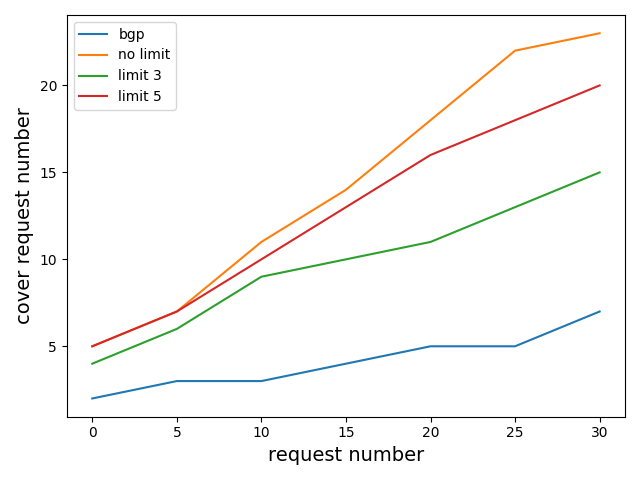
\includegraphics[width=0.46\linewidth]{./figures/ch4-test-random-topo.png}
    \label{fig-ch4-test-random-topo}
}
\\
\hspace{0.00\linewidth}
\subfloat[段路由标签列表长度分布结果图]{
    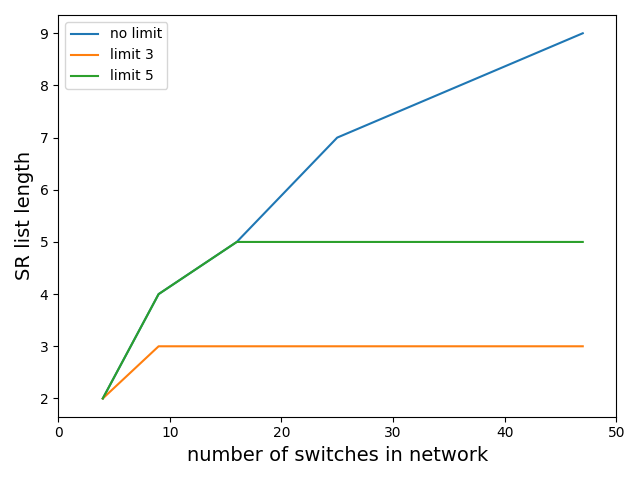
\includegraphics[width=0.46\linewidth]{./figures/ch4-sl-length.png}
    \label{fig-sl-length}
}
\hspace{0.00\linewidth}
\subfloat[基于差分时延的路径选择算法和最短路径算法的跳数对比结果图]{
    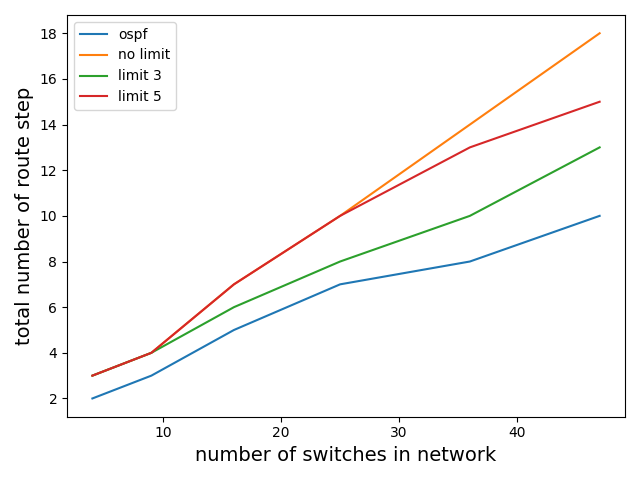
\includegraphics[width=0.46\linewidth]{./figures/ch4-total-length.png}
    \label{fig-total-length}
}
\caption{分布式段路由航点列表生成算法实验结果图} 
\label{fig:test:distributed}
\end{figure*}

图5-6是分布式段路由航点生成算法针对时延保障效果和段路由列表长度的实验结果。

\begin{itemize}
\item (a)是树状拓扑下与边界网关协议对时延需求保障的比较实验结果图。本实验是为了验证在同样使用数据中心树状拓扑的前提下,采用第四章提出的保障时延的分布式段路由航点标签列表生成算法是否比边界网关协议有更好的时延需求保障能力。在第三章提到的算法中分析了段路由列表太长会带来的问题,并且建议不要使用过长的段路由列表,而在第四章的算法中,具有对段路由标签长度进行限制和不进行限制的两种可选项,因此本实验将测试对段路由标签列表长度进行限制是否会大幅度影响路由调度的实验保障结果。本实验的自变量是服务请求的数目,这些服务请求到达时会携带一个期望的时延需求,因此用服务请求数目做为横坐标,因变量是可以满足时延需求的请求的数目,并将其在纵坐标上描点。本实验的对照组为运行边界网关协议和运行不限制标签列表长度的第四章算法下,流量对时延结果的保障情况。分析实验结果数据可以初步得出结论:第四章提出的分布式段路由航点标签列表生成算法确实比平常使用的分布式协议更能较好地保障业务的时延需求,段路由标签列表长度限制在3的时候,也可以达到较好的时延保障效果。
\item (b)是随机拓扑下与边界网关协议对时延需求保障的比较实验结果图。本实验与实验(a)类似,区别是将实验拓扑设置为模拟运营商网络的随机拓扑。本实验的自变量是在随机网络拓扑中携带目标时延发起服务请求的请求数目,并用该服务请求数目做为横坐标,纵坐标为可以满足其对应时延需求的服务请求的数目。本实验的对照组为运行边界网关协议和运行不限制标签列表长度的第四章算法下,流量对时延结果的保障情况。通过分析实验结论数据可以得出结论,第四章提出的分布式段路由航点标签列表生成算法在模拟运营商网络的随机网络拓扑中也能比其他路由协议更好地保障业务流量的时延需求,而段路由标签列表长度限制在5的时候,也可以达到和不限制下相当的较好的时延保障效果。
\item (c)是基于差分时延的路径选择算法对段路由标签列表长度分布实验验证结果图。该实验旨在验证,当不对段路由标签列表长度进行限制的情况下,第四章算法生成的段路由标签列表长度会因网络规模的扩大而增加,因此本实验主要是验证算法生成的段路由标签列表长度随着网络规模的扩大会呈现怎样的分布。本实验自变量时网络中段路由节点的数目,纵坐标因变量则是10个服务请求下计算出段路由航点列表的平均长度,对照组有对标签列表长度进行限制的算法结果段路由航点列表的平均长度。由实验结果可以看出,在不加限制的情况下段路由标签列表会和网络拓扑大小基本成线性增长,而限制段路由航点列表长度则会将标签列表长度固定,因此得出结论本算法需要根据具体网络拓扑情况,在生成段路由标签列表的时候对列表长度进行限制。
\item (d)是基于差分时延的路径选择算法和最短路径算法的跳数对比实验验证结果图。本实验目的是对比第四章提出算法的流量路径跳数是否过高,因为跳数过多会对网络带来较大的额外带宽开销,本实验自变量是网络中总节点的数目,因变量是报文在第四章段路由航点列表生成算法得到的段路由列表指导下平均总跳数,对照组时同样拓扑和同样流量服务需求下,按照开放最短路径优先协议进行流量转发最终经历的总跳数的平均值。由实验结果可以看出,在不加限制的情况下段路由标签列表指导下的路由跳数会和网络拓扑直径大小基本成线性增长,并且总跳数比开放最短路径优先协议多4.7\%到23.5\%,而开放最短路径优先协议下的总跳数总是基本和网络直径相当。
\end{itemize}

\subsection{算法结论}

通过实验验证得到:本文提出的集中式算法比对照组在数据中心网络中的流量调度时延降低了8.22\%;在运营商网络中的流量调度时延降低了3.34\%;本文提出的分布式算法在损失一定网络吞吐量的情况下,比对照组在数据中心网络中的流量调度时延下降低了53.3\%;在运营商网络中的流量调度时延降低了65.6\%。并且由于段路由航点列表长度的限制,两种算法均不会对网络造成过大的吞吐率损失。实验结果表明,基于时延信息进行段路由航点列表的计算可以降低数据中心网络和运营商网络下流量的端到端时延,为时延敏感业务提供网络层的技术支持。

\section{本章小结}

本章基于可编程的 \gls*{P4} 软件交换机 \gls*{BMv2} ,进行了基本段路由功能测试和组网流量调度实验测试。在基本段路由功能测试中主要针对 \gls*{BMv2} 的段路由功能进行测试,该实验组建了三节点线性拓扑,在三个节点上分别验证了段路由包头和段列表的封装、段路由包头弹出、段路由转发功能,证明该软件交换机足以仿真段路由功能。组网流量调度实验测试则是对第三章和第四章两种算法进行分别测试,验证其在时延保障上的能力,为更广泛地验证算法效果,在两种算法下都分别了搭建数据中心拓扑和运营商拓扑,并选定了当前常用的路由算法作为对照组。实验结果表明,集中式和分布式的段路由航点生成算法都可以有效降低流量端到端时延,为使用流量调度满足时延敏感业务的需求提供了参考。

% 测试所有参考文献类型\cite{CITATION_BOOK,CITATION_ARTICLE,CITATION_PROCEEDINGS,CITATION_INPROCEEDINGS,CITATION_TECHREPORT,CITATION_STANDARD,CITATION_PATENT,CITATION_NEWSPAPER,CITATION_ELECTRONIC,SRSURVEYS}。

%% 本章参考文献
\ifx\usechapbib\empty
\nocite{BSTcontrol}
\setcounter{NAT@ctr}{0}
\bibliographystyle{buptgraduatethesis}
\bibliography{bare_thesis}
\fi
